\documentclass[aspectratio=169]{beamer}

% Minimal theme
\usetheme{default}
\usecolortheme{dove}

% Remove navigation symbols
\setbeamertemplate{navigation symbols}{}
\setbeamertemplate{footline}{%
  \hfill{\large\insertframenumber\,/\,\inserttotalframenumber}\hspace{0.8em}\vspace{0.5em}%
}

% Colors
\definecolor{popblue}{RGB}{52, 101, 164}
\definecolor{sampred}{RGB}{204, 0, 0}
\definecolor{paramgreen}{RGB}{0, 140, 70}
\definecolor{lightbg}{RGB}{245, 245, 250}
\definecolor{warnred}{RGB}{180, 40, 40}
\definecolor{orange1}{RGB}{220, 120, 0}
\definecolor{violet1}{RGB}{120, 50, 160}

\setbeamercolor{frametitle}{fg=popblue}
\setbeamercolor{title}{fg=popblue}

% Packages
\usepackage{pgfplots}
\usepackage{tikz}
\usetikzlibrary{shapes, arrows.meta, positioning, calc, decorations.pathreplacing, patterns, fit}
\pgfplotsset{compat=1.18}
\usepackage{amsmath, amssymb}
\usepackage{array}
\usepackage{fontenc}

\title{Reasoning \& Test-Time Compute}
\subtitle{Chain-of-Thought $\cdot$ Search $\cdot$ Verification $\cdot$ Scaling Inference}
\date{}

\begin{document}

% ============================================================
% TITLE
% ============================================================
\begin{frame}
\titlepage
\end{frame}

% ============================================================
% THE TWO SCALING AXES
% ============================================================
\begin{frame}
\frametitle{The two scaling axes}

\begin{center}
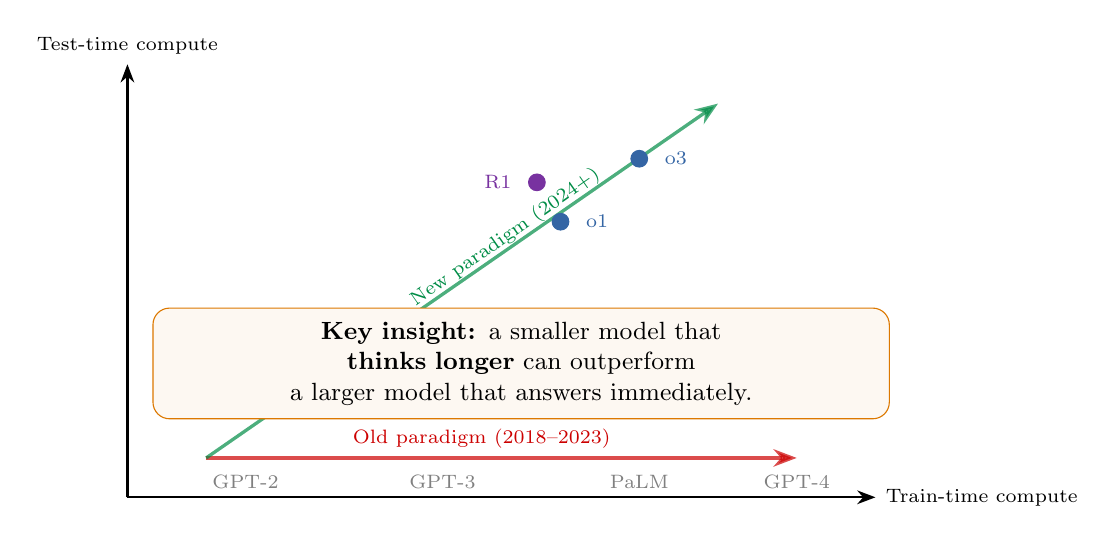
\begin{tikzpicture}
  % Axes
  \draw[-Stealth, thick] (-5, -2.5) -- (4.5, -2.5) node[right, font=\scriptsize] {Train-time compute};
  \draw[-Stealth, thick] (-5, -2.5) -- (-5, 3) node[above, font=\scriptsize] {Test-time compute};

  % Old paradigm arrow (horizontal)
  \draw[-Stealth, very thick, sampred, opacity=0.7] (-4, -2) -- (3.5, -2);
  \node[font=\scriptsize, text=sampred, above] at (-0.5, -2) {Old paradigm (2018--2023)};
  \node[font=\scriptsize, text=gray] at (-3.5, -2.3) {GPT-2};
  \node[font=\scriptsize, text=gray] at (-1, -2.3) {GPT-3};
  \node[font=\scriptsize, text=gray] at (1.5, -2.3) {PaLM};
  \node[font=\scriptsize, text=gray] at (3.5, -2.3) {GPT-4};

  % New paradigm arrow (diagonal)
  \draw[-Stealth, very thick, paramgreen, opacity=0.7] (-4, -2) -- (2.5, 2.5);
  \node[font=\scriptsize, text=paramgreen, rotate=35] at (-0.2, 0.8) {New paradigm (2024+)};

  % Key models on new axis
  \filldraw[popblue] (0.5, 1) circle (3pt);
  \node[font=\scriptsize, text=popblue, right] at (0.7, 1) {o1};
  \filldraw[popblue] (1.5, 1.8) circle (3pt);
  \node[font=\scriptsize, text=popblue, right] at (1.7, 1.8) {o3};
  \filldraw[violet1] (0.2, 1.5) circle (3pt);
  \node[font=\scriptsize, text=violet1, left] at (0.0, 1.5) {R1};

  % Key insight
  \node[draw=orange1, fill=orange1!5, rounded corners=6pt, text width=9cm, align=center, inner sep=5pt, font=\small] at (0, -0.8) {
    \textbf{Key insight:} a smaller model that \textbf{thinks longer} can outperform\\
    a larger model that answers immediately.
  };
\end{tikzpicture}
\end{center}
\end{frame}

% ============================================================
% CHAIN-OF-THOUGHT PROMPTING
% ============================================================
\begin{frame}
\frametitle{Chain-of-Thought prompting}

\begin{center}
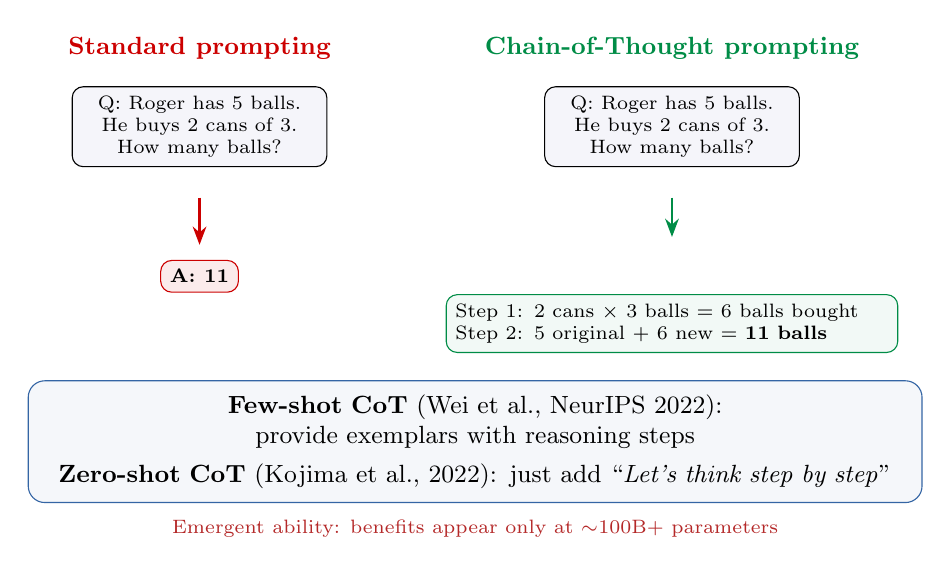
\begin{tikzpicture}
  % Standard prompting
  \node[font=\small\bfseries, text=sampred] at (-4.5, 3) {Standard prompting};
  \node[draw, rounded corners=4pt, fill=lightbg, font=\scriptsize, text width=3cm, align=center] (sq) at (-4.5, 2) {Q: Roger has 5 balls.\\He buys 2 cans of 3.\\How many balls?};
  \draw[-Stealth, thick, sampred] (-4.5, 1.1) -- (-4.5, 0.5);
  \node[draw=sampred, rounded corners=4pt, fill=sampred!8, font=\scriptsize\bfseries] at (-4.5, 0.1) {A: 11};

  % CoT prompting
  \node[font=\small\bfseries, text=paramgreen] at (1.5, 3) {Chain-of-Thought prompting};
  \node[draw, rounded corners=4pt, fill=lightbg, font=\scriptsize, text width=3cm, align=center] (cq) at (1.5, 2) {Q: Roger has 5 balls.\\He buys 2 cans of 3.\\How many balls?};
  \draw[-Stealth, thick, paramgreen] (1.5, 1.1) -- (1.5, 0.6);
  \node[draw=paramgreen, rounded corners=4pt, fill=paramgreen!5, font=\scriptsize, text width=5.5cm, align=left] at (1.5, -0.5) {
    Step 1: 2 cans $\times$ 3 balls = 6 balls bought\\
    Step 2: 5 original + 6 new = \textbf{11 balls}
  };

  % Papers
  \node[draw=popblue, fill=popblue!5, rounded corners=6pt, text width=11cm, align=center, inner sep=5pt, font=\small] at (-1, -2) {
    \textbf{Few-shot CoT} (Wei et al., NeurIPS 2022): provide exemplars with reasoning steps\\[3pt]
    \textbf{Zero-shot CoT} (Kojima et al., 2022): just add ``\textit{Let's think step by step}''
  };

  % Emergent
  \node[font=\scriptsize, text=warnred] at (-1, -3.1) {Emergent ability: benefits appear only at $\sim$100B+ parameters};
\end{tikzpicture}
\end{center}
\end{frame}

% ============================================================
% WHY COT WORKS
% ============================================================
\begin{frame}
\frametitle{Why Chain-of-Thought works}

\begin{center}
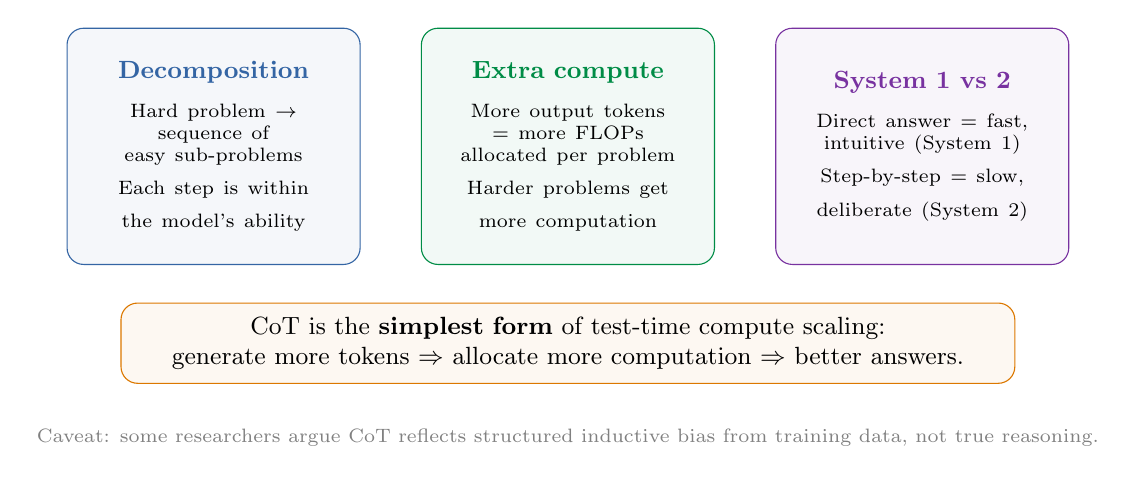
\begin{tikzpicture}
  % Three mechanism boxes
  \node[draw=popblue, fill=popblue!5, rounded corners=6pt, text width=3.3cm, align=center, inner sep=6pt, minimum height=3cm] at (-4.5, 1) {
    {\small\bfseries\textcolor{popblue}{Decomposition}}\\[6pt]
    {\scriptsize Hard problem $\to$\\sequence of\\easy sub-problems\\[4pt]
    Each step is within\\the model's ability}
  };

  \node[draw=paramgreen, fill=paramgreen!5, rounded corners=6pt, text width=3.3cm, align=center, inner sep=6pt, minimum height=3cm] at (0, 1) {
    {\small\bfseries\textcolor{paramgreen}{Extra compute}}\\[6pt]
    {\scriptsize More output tokens\\= more FLOPs\\allocated per problem\\[4pt]
    Harder problems get\\more computation}
  };

  \node[draw=violet1, fill=violet1!5, rounded corners=6pt, text width=3.3cm, align=center, inner sep=6pt, minimum height=3cm] at (4.5, 1) {
    {\small\bfseries\textcolor{violet1}{System 1 vs 2}}\\[6pt]
    {\scriptsize Direct answer = fast,\\intuitive (System 1)\\[4pt]
    Step-by-step = slow,\\deliberate (System 2)}
  };

  % Bottom insight
  \node[draw=orange1, fill=orange1!5, rounded corners=6pt, text width=11cm, align=center, inner sep=5pt, font=\small] at (0, -1.5) {
    CoT is the \textbf{simplest form} of test-time compute scaling:\\
    generate more tokens $\Rightarrow$ allocate more computation $\Rightarrow$ better answers.
  };

  \node[font=\scriptsize, text=gray] at (0, -2.7) {Caveat: some researchers argue CoT reflects structured inductive bias from training data, not true reasoning.};
\end{tikzpicture}
\end{center}
\end{frame}

% ============================================================
% SELF-CONSISTENCY
% ============================================================
\begin{frame}
\frametitle{Self-Consistency}
\vspace{-0.2cm}
\begin{center}
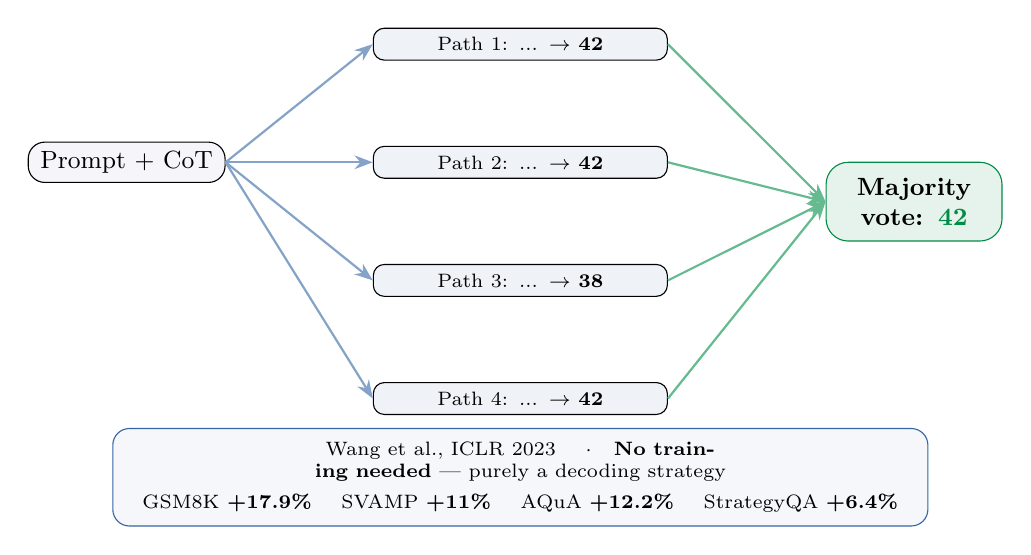
\begin{tikzpicture}
  % Prompt
  \node[draw, rounded corners=6pt, fill=lightbg, font=\small, minimum width=2.5cm] (prompt) at (-5, 1.5) {Prompt + CoT};

  % Fan out
  \node[draw, rounded corners=4pt, fill=popblue!8, font=\scriptsize, text width=3.5cm, align=center] (pA) at (0, 3) {Path 1: ... $\to$ \textbf{42}};
  \node[draw, rounded corners=4pt, fill=popblue!8, font=\scriptsize, text width=3.5cm, align=center] (pB) at (0, 1.5) {Path 2: ... $\to$ \textbf{42}};
  \node[draw, rounded corners=4pt, fill=popblue!8, font=\scriptsize, text width=3.5cm, align=center] (pC) at (0, 0) {Path 3: ... $\to$ \textbf{38}};
  \node[draw, rounded corners=4pt, fill=popblue!8, font=\scriptsize, text width=3.5cm, align=center] (pD) at (0, -1.5) {Path 4: ... $\to$ \textbf{42}};
  \draw[-Stealth, thick, popblue!60] (prompt.east) -- (pA.west);
  \draw[-Stealth, thick, popblue!60] (prompt.east) -- (pB.west);
  \draw[-Stealth, thick, popblue!60] (prompt.east) -- (pC.west);
  \draw[-Stealth, thick, popblue!60] (prompt.east) -- (pD.west);

  % Majority vote
  \node[draw=paramgreen, fill=paramgreen!10, rounded corners=8pt, font=\small\bfseries, text width=2cm, align=center, minimum height=1cm] (vote) at (5, 1) {Majority\\vote: \textcolor{paramgreen}{42}};
  \draw[-Stealth, thick, paramgreen!60] (pA.east) -- (vote.west);
  \draw[-Stealth, thick, paramgreen!60] (pB.east) -- (vote.west);
  \draw[-Stealth, thick, paramgreen!60] (pC.east) -- (vote.west);
  \draw[-Stealth, thick, paramgreen!60] (pD.east) -- (vote.west);

  % Results table
  \node[draw=popblue, fill=popblue!5, rounded corners=6pt, text width=10cm, align=center, inner sep=5pt, font=\scriptsize] at (0, -2.5) {
    Wang et al., ICLR 2023 \quad$\cdot$\quad \textbf{No training needed} --- purely a decoding strategy\\[3pt]
    GSM8K \textbf{+17.9\%} \quad SVAMP \textbf{+11\%} \quad AQuA \textbf{+12.2\%} \quad StrategyQA \textbf{+6.4\%}
  };
\end{tikzpicture}
\end{center}
\end{frame}

% ============================================================
% TREE OF THOUGHTS
% ============================================================
\begin{frame}
\frametitle{Tree of Thoughts}

\begin{center}
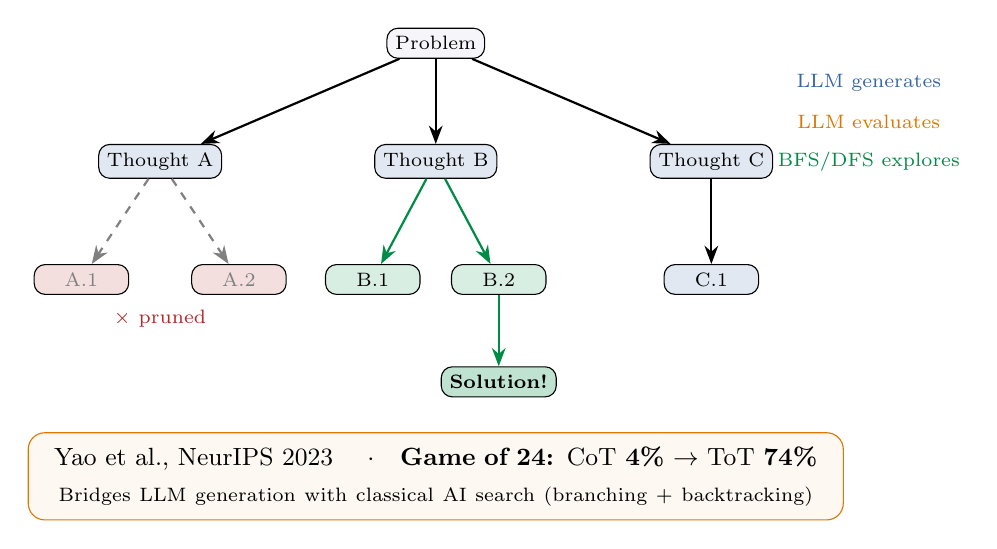
\begin{tikzpicture}
  % Root
  \node[draw, rounded corners=4pt, fill=lightbg, font=\scriptsize, minimum width=1.2cm, inner sep=3pt, align=center] (root) at (0, 3) {Problem};

  % Level 1
  \node[draw, rounded corners=4pt, fill=popblue!15, font=\scriptsize, minimum width=1.2cm, inner sep=3pt, align=center] (a) at (-3.5, 1.5) {Thought A};
  \node[draw, rounded corners=4pt, fill=popblue!15, font=\scriptsize, minimum width=1.2cm, inner sep=3pt, align=center] (b) at (0, 1.5) {Thought B};
  \node[draw, rounded corners=4pt, fill=popblue!15, font=\scriptsize, minimum width=1.2cm, inner sep=3pt, align=center] (c) at (3.5, 1.5) {Thought C};
  \draw[-Stealth, thick] (root) -- (a);
  \draw[-Stealth, thick] (root) -- (b);
  \draw[-Stealth, thick] (root) -- (c);

  % Level 2 from A (pruned)
  \node[draw, rounded corners=4pt, fill=warnred!15, font=\scriptsize, text=gray, minimum width=1.2cm, inner sep=3pt, align=center] (a1) at (-4.5, 0) {A.1};
  \node[draw, rounded corners=4pt, fill=warnred!15, font=\scriptsize, text=gray, minimum width=1.2cm, inner sep=3pt, align=center] (a2) at (-2.5, 0) {A.2};
  \draw[-Stealth, thick, gray, dashed] (a) -- (a1);
  \draw[-Stealth, thick, gray, dashed] (a) -- (a2);
  \node[font=\scriptsize, text=warnred] at (-3.5, -0.5) {\texttimes\ pruned};

  % Level 2 from B (continues)
  \node[draw, rounded corners=4pt, fill=paramgreen!15, font=\scriptsize, minimum width=1.2cm, inner sep=3pt, align=center] (b1) at (-0.8, 0) {B.1};
  \node[draw, rounded corners=4pt, fill=paramgreen!15, font=\scriptsize, minimum width=1.2cm, inner sep=3pt, align=center] (b2) at (0.8, 0) {B.2};
  \draw[-Stealth, thick, paramgreen] (b) -- (b1);
  \draw[-Stealth, thick, paramgreen] (b) -- (b2);

  % Level 3 from B.2 (solution)
  \node[draw, rounded corners=4pt, fill=paramgreen!25, font=\scriptsize\bfseries, minimum width=1.2cm, inner sep=3pt, align=center] (sol) at (0.8, -1.3) {Solution!};
  \draw[-Stealth, thick, paramgreen] (b2) -- (sol);

  % Level 2 from C
  \node[draw, rounded corners=4pt, fill=popblue!15, font=\scriptsize, minimum width=1.2cm, inner sep=3pt, align=center] (c1) at (3.5, 0) {C.1};
  \draw[-Stealth, thick] (c) -- (c1);

  % Labels
  \node[font=\scriptsize, text=popblue] at (5.5, 2.5) {LLM generates};
  \node[font=\scriptsize, text=orange1] at (5.5, 2) {LLM evaluates};
  \node[font=\scriptsize, text=paramgreen] at (5.5, 1.5) {BFS/DFS explores};

  % Bottom
  \node[draw=orange1, fill=orange1!5, rounded corners=6pt, text width=10cm, align=center, inner sep=5pt, font=\small] at (0, -2.5) {
    Yao et al., NeurIPS 2023 \quad$\cdot$\quad \textbf{Game of 24:} CoT \textbf{4\%} $\to$ ToT \textbf{74\%}\\[2pt]
    {\scriptsize Bridges LLM generation with classical AI search (branching + backtracking)}
  };
\end{tikzpicture}
\end{center}
\end{frame}

% ============================================================
% PROCESS VS OUTCOME REWARD MODELS
% ============================================================
\begin{frame}
\frametitle{Process vs.\ Outcome Reward Models}

\begin{center}
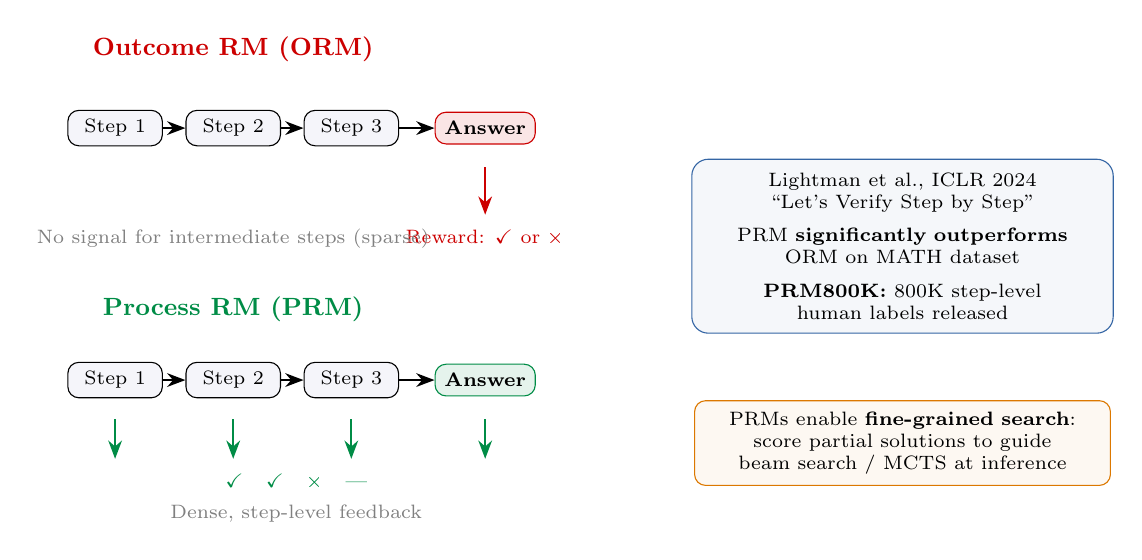
\begin{tikzpicture}
  % ORM pipeline
  \node[font=\small\bfseries, text=sampred] at (-4, 3) {Outcome RM (ORM)};
  \node[draw, rounded corners=4pt, fill=lightbg, font=\scriptsize, minimum width=1.2cm] (os1) at (-5.5, 2) {Step 1};
  \node[draw, rounded corners=4pt, fill=lightbg, font=\scriptsize, minimum width=1.2cm] (os2) at (-4, 2) {Step 2};
  \node[draw, rounded corners=4pt, fill=lightbg, font=\scriptsize, minimum width=1.2cm] (os3) at (-2.5, 2) {Step 3};
  \draw[-Stealth, thick] (os1) -- (os2);
  \draw[-Stealth, thick] (os2) -- (os3);
  \node[draw=sampred, rounded corners=4pt, fill=sampred!10, font=\scriptsize\bfseries] (oans) at (-0.8, 2) {Answer};
  \draw[-Stealth, thick] (os3) -- (oans);
  % Only final reward
  \draw[-Stealth, thick, sampred] (-0.8, 1.5) -- (-0.8, 0.9);
  \node[font=\scriptsize, text=sampred] at (-0.8, 0.6) {Reward: \checkmark\ or \texttimes};
  \node[font=\scriptsize, text=gray] at (-4, 0.6) {No signal for intermediate steps (sparse)};

  % PRM pipeline
  \node[font=\small\bfseries, text=paramgreen] at (-4, -0.3) {Process RM (PRM)};
  \node[draw, rounded corners=4pt, fill=lightbg, font=\scriptsize, minimum width=1.2cm] (ps1) at (-5.5, -1.2) {Step 1};
  \node[draw, rounded corners=4pt, fill=lightbg, font=\scriptsize, minimum width=1.2cm] (ps2) at (-4, -1.2) {Step 2};
  \node[draw, rounded corners=4pt, fill=lightbg, font=\scriptsize, minimum width=1.2cm] (ps3) at (-2.5, -1.2) {Step 3};
  \node[draw=paramgreen, rounded corners=4pt, fill=paramgreen!10, font=\scriptsize\bfseries] (pans) at (-0.8, -1.2) {Answer};
  \draw[-Stealth, thick] (ps1) -- (ps2);
  \draw[-Stealth, thick] (ps2) -- (ps3);
  \draw[-Stealth, thick] (ps3) -- (pans);
  % Step-level rewards
  \draw[-Stealth, thick, paramgreen] (-5.5, -1.7) -- (-5.5, -2.2);
  \draw[-Stealth, thick, paramgreen] (-4, -1.7) -- (-4, -2.2);
  \draw[-Stealth, thick, paramgreen] (-2.5, -1.7) -- (-2.5, -2.2);
  \draw[-Stealth, thick, paramgreen] (-0.8, -1.7) -- (-0.8, -2.2);
  \node[font=\scriptsize, text=paramgreen] at (-3.2, -2.5) {\checkmark\quad \checkmark\quad \texttimes\quad ---};
  \node[font=\scriptsize, text=gray] at (-3.2, -2.9) {Dense, step-level feedback};

  % Key results box
  \node[draw=popblue, fill=popblue!5, rounded corners=6pt, text width=5cm, align=center, inner sep=5pt, font=\scriptsize] at (4.5, 0.5) {
    Lightman et al., ICLR 2024\\``Let's Verify Step by Step''\\[4pt]
    PRM \textbf{significantly outperforms}\\ORM on MATH dataset\\[4pt]
    \textbf{PRM800K:} 800K step-level\\human labels released
  };

  \node[draw=orange1, fill=orange1!5, rounded corners=4pt, text width=5cm, align=center, inner sep=4pt, font=\scriptsize] at (4.5, -2) {
    PRMs enable \textbf{fine-grained search}:\\score partial solutions to guide\\beam search / MCTS at inference
  };
\end{tikzpicture}
\end{center}
\end{frame}

% ============================================================
% SEARCH AT INFERENCE TIME
% ============================================================
\begin{frame}
\frametitle{Search at inference time}
\vspace{-0.2cm}
\begin{center}
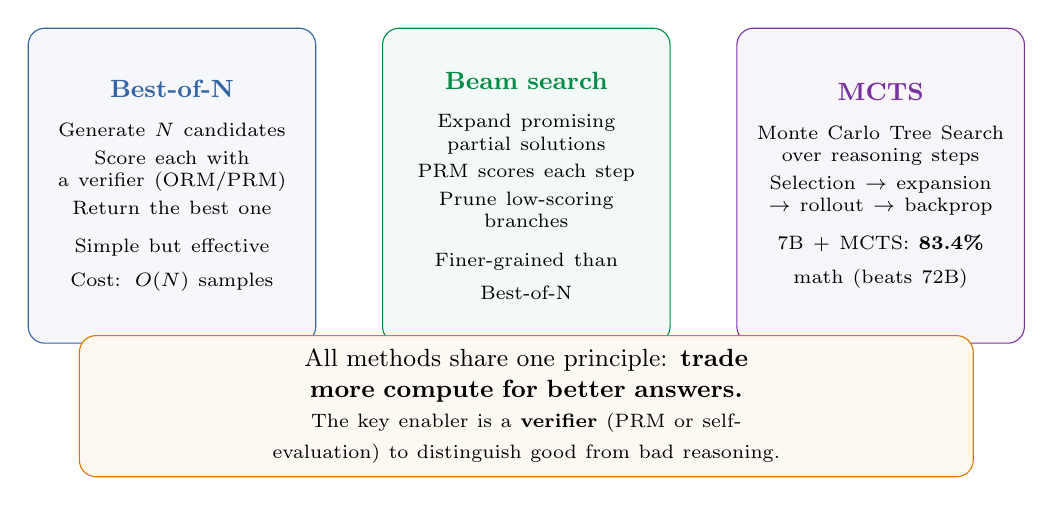
\begin{tikzpicture}
  % Best-of-N
  \node[draw=popblue, fill=popblue!5, rounded corners=6pt, text width=3.3cm, align=center, inner sep=5pt, minimum height=4cm] at (-4.5, 0.8) {
    {\small\bfseries\textcolor{popblue}{Best-of-N}}\\[6pt]
    {\scriptsize Generate $N$ candidates\\[2pt]
    Score each with\\a verifier (ORM/PRM)\\[2pt]
    Return the best one\\[6pt]
    Simple but effective\\
    Cost: $O(N)$ samples}
  };

  % Beam search
  \node[draw=paramgreen, fill=paramgreen!5, rounded corners=6pt, text width=3.3cm, align=center, inner sep=5pt, minimum height=4cm] at (0, 0.8) {
    {\small\bfseries\textcolor{paramgreen}{Beam search}}\\[6pt]
    {\scriptsize Expand promising\\partial solutions\\[2pt]
    PRM scores each step\\[2pt]
    Prune low-scoring\\branches\\[6pt]
    Finer-grained than\\Best-of-N}
  };

  % MCTS
  \node[draw=violet1, fill=violet1!5, rounded corners=6pt, text width=3.3cm, align=center, inner sep=5pt, minimum height=4cm] at (4.5, 0.8) {
    {\small\bfseries\textcolor{violet1}{MCTS}}\\[6pt]
    {\scriptsize Monte Carlo Tree Search\\over reasoning steps\\[2pt]
    Selection $\to$ expansion\\$\to$ rollout $\to$ backprop\\[6pt]
    7B + MCTS: \textbf{83.4\%}\\math (beats 72B)}
  };

  % Bottom insight
  \node[draw=orange1, fill=orange1!5, rounded corners=6pt, text width=11cm, align=center, inner sep=5pt, font=\small] at (0, -2) {
    All methods share one principle: \textbf{trade more compute for better answers.}\\
    {\scriptsize The key enabler is a \textbf{verifier} (PRM or self-evaluation) to distinguish good from bad reasoning.}
  };
\end{tikzpicture}
\end{center}
\end{frame}

% ============================================================
% TEST-TIME COMPUTE SCALING LAWS
% ============================================================
\begin{frame}
\frametitle{Test-time compute scaling laws}
\vspace{-0.2cm}
\begin{center}
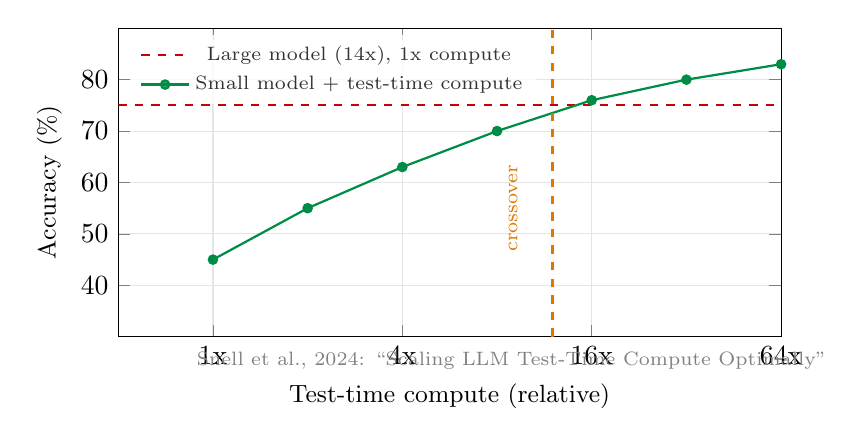
\begin{tikzpicture}
  \begin{axis}[
    width=10cm, height=5.5cm,
    xlabel={\small Test-time compute (relative)},
    ylabel={\small Accuracy (\%)},
    xmin=0.5, xmax=64,
    ymin=30, ymax=90,
    xmode=log,
    log basis x=2,
    xtick={1, 4, 16, 64},
    xticklabels={1x, 4x, 16x, 64x},
    ytick={40, 50, 60, 70, 80},
    grid=major,
    grid style={gray!20},
    legend style={at={(0.02,0.98)}, anchor=north west, font=\scriptsize, draw=none, fill=white, fill opacity=0.8},
  ]
    % Large model baseline (flat)
    \addplot[thick, sampred, dashed, domain=0.5:64, samples=2] {75};
    \addlegendentry{Large model (14x), 1x compute}

    % Small model with scaling test-time compute
    \addplot[thick, paramgreen, mark=*, mark size=1.5pt] coordinates {
      (1, 45) (2, 55) (4, 63) (8, 70) (16, 76) (32, 80) (64, 83)
    };
    \addlegendentry{Small model + test-time compute}

    % Crossing point annotation
    \draw[thick, orange1, dashed] (axis cs:12, 30) -- (axis cs:12, 90);
    \node[font=\scriptsize, text=orange1, rotate=90] at (axis cs:9, 55) {crossover};
  \end{axis}

  % Citation
  \node[font=\scriptsize, text=gray] at (5, -0.3) {Snell et al., 2024: ``Scaling LLM Test-Time Compute Optimally''};
\end{tikzpicture}
\end{center}
\end{frame}

% ============================================================
% OPENAI O1
% ============================================================
\begin{frame}
\frametitle{OpenAI o1: reasoning via reinforcement learning}

\begin{center}
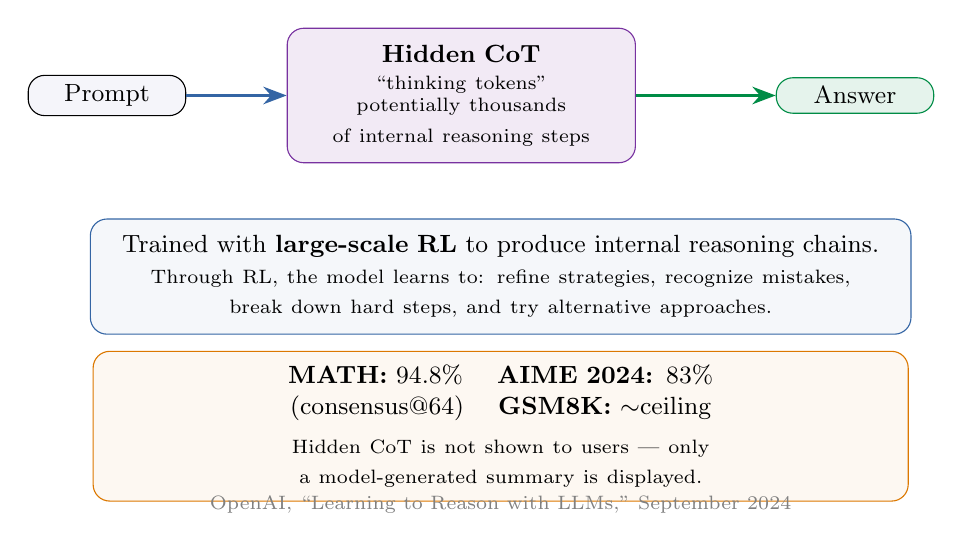
\begin{tikzpicture}
  % Pipeline
  \node[draw, rounded corners=6pt, fill=lightbg, font=\small, minimum width=2cm] (prompt) at (-5.5, 2) {Prompt};

  \node[draw=violet1, fill=violet1!10, rounded corners=6pt, font=\small, text width=4cm, align=center, inner sep=6pt] (think) at (-1, 2) {
    \textbf{Hidden CoT}\\[2pt]
    {\scriptsize ``thinking tokens''\\potentially thousands\\of internal reasoning steps}
  };

  \node[draw=paramgreen, fill=paramgreen!10, rounded corners=6pt, font=\small, minimum width=2cm] (answer) at (4, 2) {Answer};

  \draw[-Stealth, very thick, popblue] (prompt) -- (think);
  \draw[-Stealth, very thick, paramgreen] (think) -- (answer);

  % Training
  \node[draw=popblue, fill=popblue!5, rounded corners=6pt, text width=10cm, align=center, inner sep=6pt, font=\small] at (-0.5, -0.3) {
    Trained with \textbf{large-scale RL} to produce internal reasoning chains.\\[3pt]
    {\scriptsize Through RL, the model learns to: refine strategies, recognize mistakes,\\
    break down hard steps, and try alternative approaches.}
  };

  % Benchmarks
  \node[draw=orange1, fill=orange1!5, rounded corners=6pt, text width=10cm, align=center, inner sep=5pt, font=\small] at (-0.5, -2.2) {
    \textbf{MATH:} 94.8\% \quad \textbf{AIME 2024:} 83\% (consensus@64) \quad \textbf{GSM8K:} $\sim$ceiling\\[3pt]
    {\scriptsize Hidden CoT is not shown to users --- only a model-generated summary is displayed.}
  };

  \node[font=\scriptsize, text=gray] at (-0.5, -3.2) {OpenAI, ``Learning to Reason with LLMs,'' September 2024};
\end{tikzpicture}
\end{center}
\end{frame}

% ============================================================
% OPENAI O3
% ============================================================
\begin{frame}
\frametitle{OpenAI o3: scaling inference further}
\vspace{-0.2cm}
\begin{center}
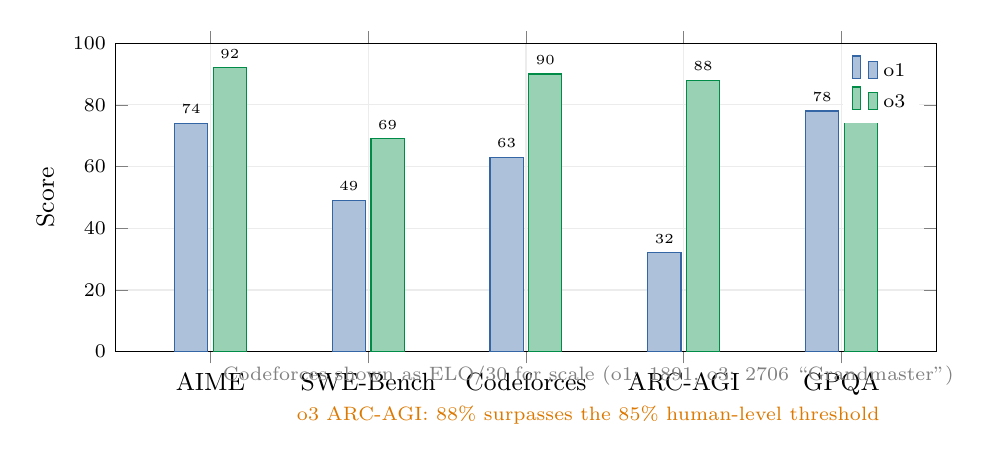
\begin{tikzpicture}
  \begin{axis}[
    width=12cm, height=5.5cm,
    ybar,
    bar width=12pt,
    ylabel={\small Score},
    symbolic x coords={AIME, SWE-Bench, Codeforces, ARC-AGI, GPQA},
    xtick=data,
    xticklabel style={font=\small},
    ymin=0, ymax=100,
    ytick={0, 20, 40, 60, 80, 100},
    yticklabel style={font=\scriptsize},
    grid=major,
    grid style={gray!15},
    legend style={at={(0.98,0.98)}, anchor=north east, font=\scriptsize, draw=none},
    enlarge x limits=0.15,
    nodes near coords,
    every node near coord/.append style={font=\tiny},
  ]
    \addplot[fill=popblue!40, draw=popblue] coordinates {
      (AIME, 74) (SWE-Bench, 49) (Codeforces, 63) (ARC-AGI, 32) (GPQA, 78)
    };
    \addlegendentry{o1}

    \addplot[fill=paramgreen!40, draw=paramgreen] coordinates {
      (AIME, 92) (SWE-Bench, 69) (Codeforces, 90) (ARC-AGI, 88) (GPQA, 88)
    };
    \addlegendentry{o3}
  \end{axis}

  % Notes
  \node[font=\scriptsize, text=gray] at (6, -0.3) {Codeforces shown as ELO/30 for scale (o1: 1891, o3: 2706 ``Grandmaster'')};
  \node[font=\scriptsize, text=orange1] at (6, -0.8) {o3 ARC-AGI: 88\% surpasses the 85\% human-level threshold};
\end{tikzpicture}
\end{center}
\end{frame}

% ============================================================
% DEEPSEEK-R1
% ============================================================
\begin{frame}
\frametitle{DeepSeek-R1: open-source reasoning}

\begin{center}
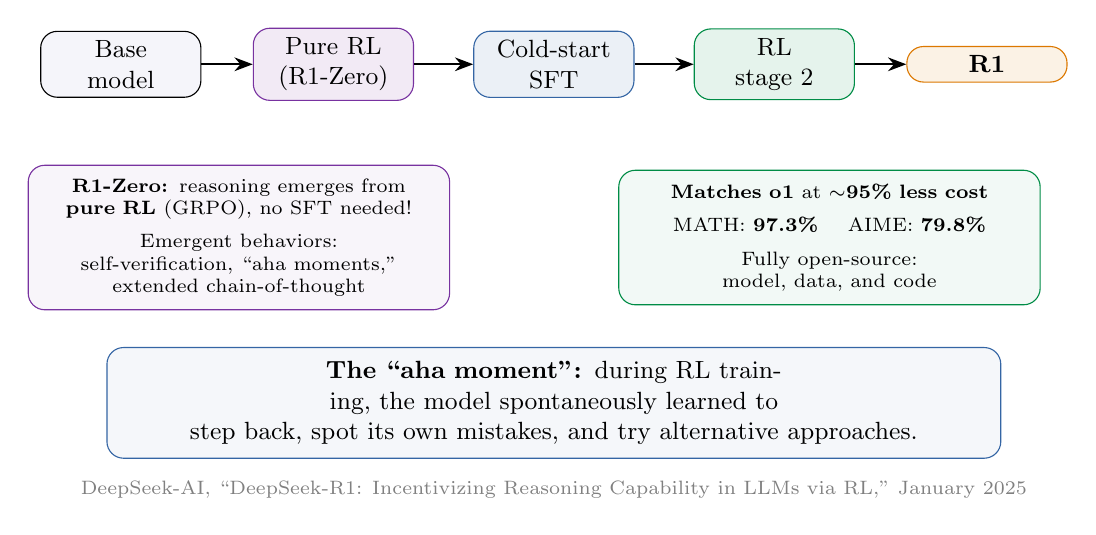
\begin{tikzpicture}
  % Pipeline boxes
  \node[draw, rounded corners=6pt, fill=lightbg, font=\small, text width=1.8cm, align=center] (base) at (-5.5, 2.5) {Base\\model};
  \node[draw=violet1, fill=violet1!10, rounded corners=6pt, font=\small, text width=1.8cm, align=center] (rl0) at (-2.8, 2.5) {Pure RL\\(R1-Zero)};
  \node[draw=popblue, fill=popblue!10, rounded corners=6pt, font=\small, text width=1.8cm, align=center] (sft) at (0, 2.5) {Cold-start\\SFT};
  \node[draw=paramgreen, fill=paramgreen!10, rounded corners=6pt, font=\small, text width=1.8cm, align=center] (rl2) at (2.8, 2.5) {RL\\stage 2};
  \node[draw=orange1, fill=orange1!10, rounded corners=6pt, font=\small\bfseries, text width=1.8cm, align=center] (r1) at (5.5, 2.5) {R1};

  \draw[-Stealth, thick] (base) -- (rl0);
  \draw[-Stealth, thick] (rl0) -- (sft);
  \draw[-Stealth, thick] (sft) -- (rl2);
  \draw[-Stealth, thick] (rl2) -- (r1);

  % Key insight: R1-Zero
  \node[draw=violet1, fill=violet1!5, rounded corners=6pt, text width=5cm, align=center, inner sep=5pt, font=\scriptsize] at (-4, 0.3) {
    \textbf{R1-Zero:} reasoning emerges from\\
    \textbf{pure RL} (GRPO), no SFT needed!\\[4pt]
    Emergent behaviors:\\self-verification, ``aha moments,''\\extended chain-of-thought
  };

  % Results
  \node[draw=paramgreen, fill=paramgreen!5, rounded corners=6pt, text width=5cm, align=center, inner sep=5pt, font=\scriptsize] at (3.5, 0.3) {
    \textbf{Matches o1} at $\sim$\textbf{95\% less cost}\\[4pt]
    MATH: \textbf{97.3\%} \quad AIME: \textbf{79.8\%}\\[4pt]
    Fully open-source:\\model, data, and code
  };

  % Bottom
  \node[draw=popblue, fill=popblue!5, rounded corners=6pt, text width=11cm, align=center, inner sep=5pt, font=\small] at (0, -1.8) {
    \textbf{The ``aha moment'':} during RL training, the model spontaneously learned to\\
    step back, spot its own mistakes, and try alternative approaches.
  };

  \node[font=\scriptsize, text=gray] at (0, -2.9) {DeepSeek-AI, ``DeepSeek-R1: Incentivizing Reasoning Capability in LLMs via RL,'' January 2025};
\end{tikzpicture}
\end{center}
\end{frame}

% ============================================================
% DISTILLATION OF REASONING
% ============================================================
\begin{frame}
\frametitle{Distillation of reasoning}

\begin{center}
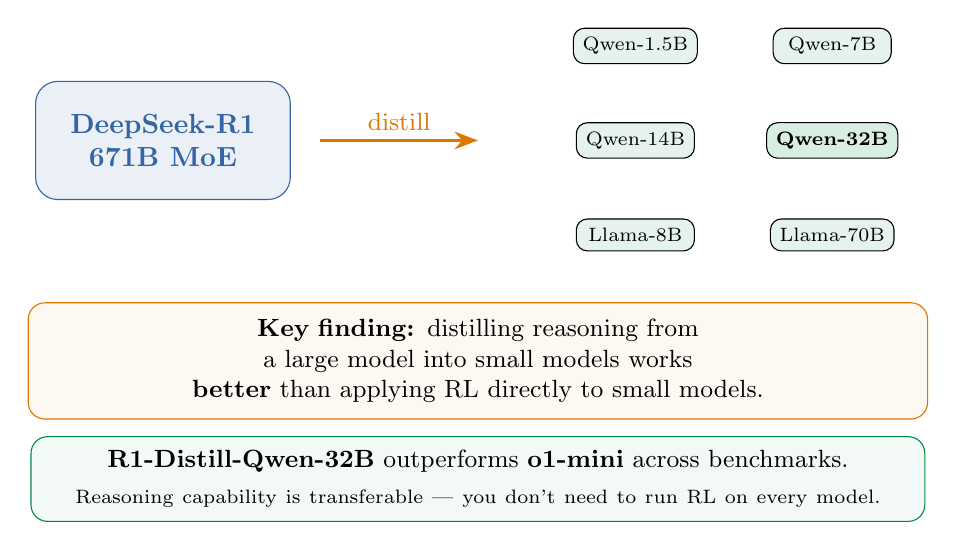
\begin{tikzpicture}
  % Large model
  \node[draw=popblue, fill=popblue!10, rounded corners=8pt, font=\normalsize\bfseries, text width=3cm, align=center, minimum height=1.5cm, text=popblue] (big) at (-4, 2) {DeepSeek-R1\\671B MoE};

  % Arrow
  \draw[-Stealth, very thick, orange1] (-2, 2) -- (0, 2);
  \node[font=\small, text=orange1, above] at (-1, 2) {distill};

  % Small models
  \node[draw, rounded corners=4pt, fill=paramgreen!10, font=\scriptsize, minimum width=1.5cm] at (2, 3.2) {Qwen-1.5B};
  \node[draw, rounded corners=4pt, fill=paramgreen!10, font=\scriptsize, minimum width=1.5cm] at (4.5, 3.2) {Qwen-7B};
  \node[draw, rounded corners=4pt, fill=paramgreen!10, font=\scriptsize, minimum width=1.5cm] at (2, 2) {Qwen-14B};
  \node[draw, rounded corners=4pt, fill=paramgreen!15, font=\scriptsize\bfseries, minimum width=1.5cm] at (4.5, 2) {Qwen-32B};
  \node[draw, rounded corners=4pt, fill=paramgreen!10, font=\scriptsize, minimum width=1.5cm] at (2, 0.8) {Llama-8B};
  \node[draw, rounded corners=4pt, fill=paramgreen!10, font=\scriptsize, minimum width=1.5cm] at (4.5, 0.8) {Llama-70B};

  % Key finding
  \node[draw=orange1, fill=orange1!5, rounded corners=6pt, text width=11cm, align=center, inner sep=6pt, font=\small] at (0, -0.8) {
    \textbf{Key finding:} distilling reasoning from a large model into small models works\\
    \textbf{better} than applying RL directly to small models.
  };

  \node[draw=paramgreen, fill=paramgreen!5, rounded corners=6pt, text width=11cm, align=center, inner sep=5pt, font=\small] at (0, -2.3) {
    \textbf{R1-Distill-Qwen-32B} outperforms \textbf{o1-mini} across benchmarks.\\[2pt]
    {\scriptsize Reasoning capability is transferable --- you don't need to run RL on every model.}
  };
\end{tikzpicture}
\end{center}
\end{frame}

% ============================================================
% BUDGET FORCING & ADAPTIVE COMPUTE
% ============================================================
\begin{frame}
\frametitle{Budget forcing \& adaptive compute}

\begin{center}
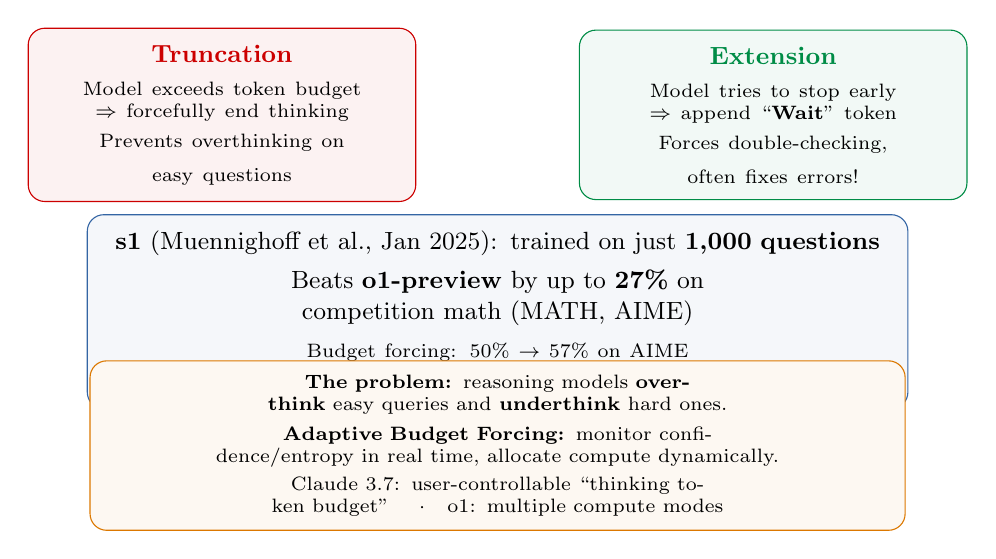
\begin{tikzpicture}
  % Truncation
  \node[draw=sampred, fill=sampred!5, rounded corners=6pt, text width=4.5cm, align=center, inner sep=6pt] at (-3.5, 2.2) {
    {\small\bfseries\textcolor{sampred}{Truncation}}\\[4pt]
    {\scriptsize Model exceeds token budget\\$\Rightarrow$ forcefully end thinking\\[3pt]
    Prevents overthinking on\\easy questions}
  };

  % Extension
  \node[draw=paramgreen, fill=paramgreen!5, rounded corners=6pt, text width=4.5cm, align=center, inner sep=6pt] at (3.5, 2.2) {
    {\small\bfseries\textcolor{paramgreen}{Extension}}\\[4pt]
    {\scriptsize Model tries to stop early\\$\Rightarrow$ append ``\textbf{Wait}'' token\\[3pt]
    Forces double-checking,\\often fixes errors!}
  };

  % s1 results
  \node[draw=popblue, fill=popblue!5, rounded corners=6pt, text width=10cm, align=center, inner sep=6pt, font=\small] at (0, -0.3) {
    \textbf{s1} (Muennighoff et al., Jan 2025): trained on just \textbf{1,000 questions}\\[3pt]
    Beats \textbf{o1-preview} by up to \textbf{27\%} on competition math (MATH, AIME)\\[3pt]
    {\scriptsize Budget forcing: 50\% $\to$ 57\% on AIME by simply letting the model think longer}
  };

  % Adaptive
  \node[draw=orange1, fill=orange1!5, rounded corners=6pt, text width=10cm, align=center, inner sep=5pt, font=\scriptsize] at (0, -2) {
    \textbf{The problem:} reasoning models \textbf{overthink} easy queries and \textbf{underthink} hard ones.\\[3pt]
    \textbf{Adaptive Budget Forcing:} monitor confidence/entropy in real time, allocate compute dynamically.\\[2pt]
    Claude 3.7: user-controllable ``thinking token budget'' \quad$\cdot$\quad o1: multiple compute modes
  };
\end{tikzpicture}
\end{center}
\end{frame}

% ============================================================
% THE REASONING LANDSCAPE (TIMELINE)
% ============================================================
\begin{frame}
\frametitle{The reasoning landscape}
\vspace{-0.2cm}
\begin{center}
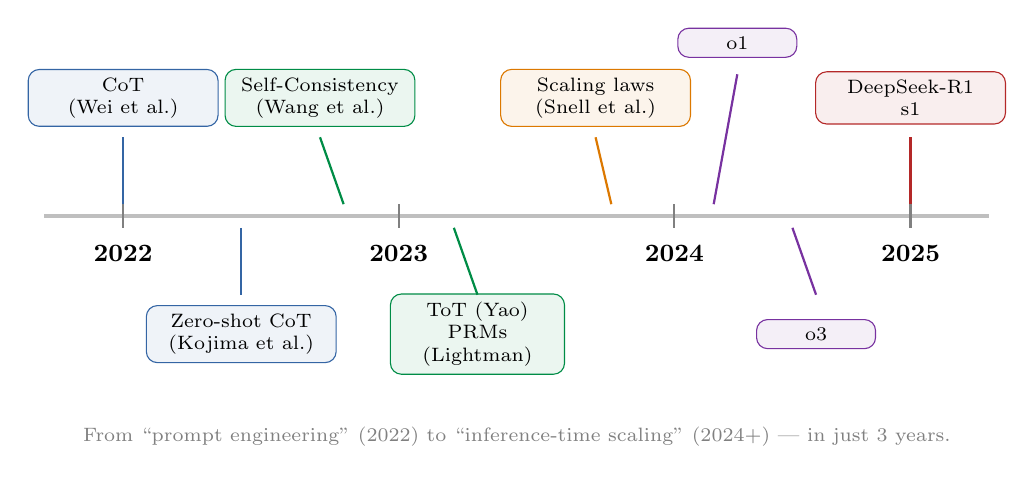
\begin{tikzpicture}
  % Timeline axis
  \draw[very thick, gray!50] (-6, 0) -- (6, 0);

  % Year markers
  \draw[thick, gray] (-5, -0.15) -- (-5, 0.15);
  \node[font=\small\bfseries, below] at (-5, -0.25) {2022};
  \draw[thick, gray] (-1.5, -0.15) -- (-1.5, 0.15);
  \node[font=\small\bfseries, below] at (-1.5, -0.25) {2023};
  \draw[thick, gray] (2, -0.15) -- (2, 0.15);
  \node[font=\small\bfseries, below] at (2, -0.25) {2024};
  \draw[thick, gray] (5, -0.15) -- (5, 0.15);
  \node[font=\small\bfseries, below] at (5, -0.25) {2025};

  % 2022 events
  \node[draw=popblue, fill=popblue!8, rounded corners=4pt, font=\scriptsize, text width=2.2cm, align=center, inner sep=3pt] at (-5, 1.5) {CoT\\(Wei et al.)};
  \draw[thick, popblue] (-5, 0.15) -- (-5, 1);
  \node[draw=popblue, fill=popblue!8, rounded corners=4pt, font=\scriptsize, text width=2.2cm, align=center, inner sep=3pt] at (-3.5, -1.5) {Zero-shot CoT\\(Kojima et al.)};
  \draw[thick, popblue] (-3.5, -0.15) -- (-3.5, -1);

  % 2023 events
  \node[draw=paramgreen, fill=paramgreen!8, rounded corners=4pt, font=\scriptsize, text width=2.2cm, align=center, inner sep=3pt] at (-2.5, 1.5) {Self-Consistency\\(Wang et al.)};
  \draw[thick, paramgreen] (-2.2, 0.15) -- (-2.5, 1);
  \node[draw=paramgreen, fill=paramgreen!8, rounded corners=4pt, font=\scriptsize, text width=2cm, align=center, inner sep=3pt] at (-0.5, -1.5) {ToT (Yao)\\PRMs (Lightman)};
  \draw[thick, paramgreen] (-0.8, -0.15) -- (-0.5, -1);

  % 2024 events
  \node[draw=orange1, fill=orange1!8, rounded corners=4pt, font=\scriptsize, text width=2.2cm, align=center, inner sep=3pt] at (1, 1.5) {Scaling laws\\(Snell et al.)};
  \draw[thick, orange1] (1.2, 0.15) -- (1, 1);
  \node[draw=violet1, fill=violet1!8, rounded corners=4pt, font=\scriptsize, text width=1.3cm, align=center, inner sep=3pt] at (2.8, 2.2) {o1};
  \draw[thick, violet1] (2.5, 0.15) -- (2.8, 1.8);
  \node[draw=violet1, fill=violet1!8, rounded corners=4pt, font=\scriptsize, text width=1.3cm, align=center, inner sep=3pt] at (3.8, -1.5) {o3};
  \draw[thick, violet1] (3.5, -0.15) -- (3.8, -1);

  % 2025 events
  \node[draw=warnred, fill=warnred!8, rounded corners=4pt, font=\scriptsize, text width=2.2cm, align=center, inner sep=3pt] at (5, 1.5) {DeepSeek-R1\\s1};
  \draw[thick, warnred] (5, 0.15) -- (5, 1);

  % Bottom
  \node[font=\scriptsize, text=gray, text width=12cm, align=center] at (0, -2.8) {
    From ``prompt engineering'' (2022) to ``inference-time scaling'' (2024+) --- in just 3 years.
  };
\end{tikzpicture}
\end{center}
\end{frame}

% ============================================================
% KEY BENCHMARKS
% ============================================================
\begin{frame}
\frametitle{Key reasoning benchmarks}
\vspace{-0.2cm}
\renewcommand{\arraystretch}{1.3}
\begin{center}
{\small
\begin{tabular}{>{\bfseries}l l l l}
\hline
\textbf{Benchmark} & \textbf{What it tests} & \textbf{Scale} & \textbf{Frontier SOTA} \\
\hline
GSM8K & Grade-school math & 1K test & \textcolor{gray}{Saturated ($>$95\%)} \\
MATH & Competition math & 5K test & R1: \textbf{97.3\%} \\
AIME & Hard competition (15 Q/yr) & 15/year & o3: \textbf{91.6\%} \\
ARC-AGI & Fluid intelligence & $\sim$400 tasks & o3: \textbf{88\%} \\
Codeforces & Competitive programming & ELO rating & o3: \textbf{2706} (GM) \\
SWE-Bench & Real GitHub issues & 2.3K tasks & o3: \textbf{69.1\%} \\
GPQA & PhD-level science & 198 Q & o3: \textbf{87.7\%} \\
\hline
\end{tabular}
}
\end{center}

\vspace{0.2cm}
\begin{center}
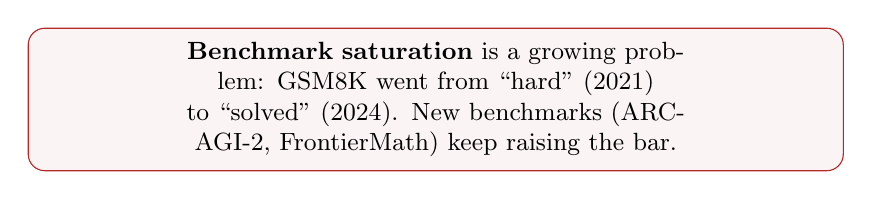
\begin{tikzpicture}
  \node[draw=warnred, fill=warnred!5, rounded corners=6pt, text width=10cm, align=center, inner sep=5pt, font=\small] at (0, 0) {
    \textbf{Benchmark saturation} is a growing problem: GSM8K went from ``hard'' (2021)\\
    to ``solved'' (2024). New benchmarks (ARC-AGI-2, FrontierMath) keep raising the bar.
  };
\end{tikzpicture}
\end{center}
\end{frame}

% ============================================================
% THE ECONOMICS OF THINKING
% ============================================================
\begin{frame}
\frametitle{The economics of thinking}

\begin{center}
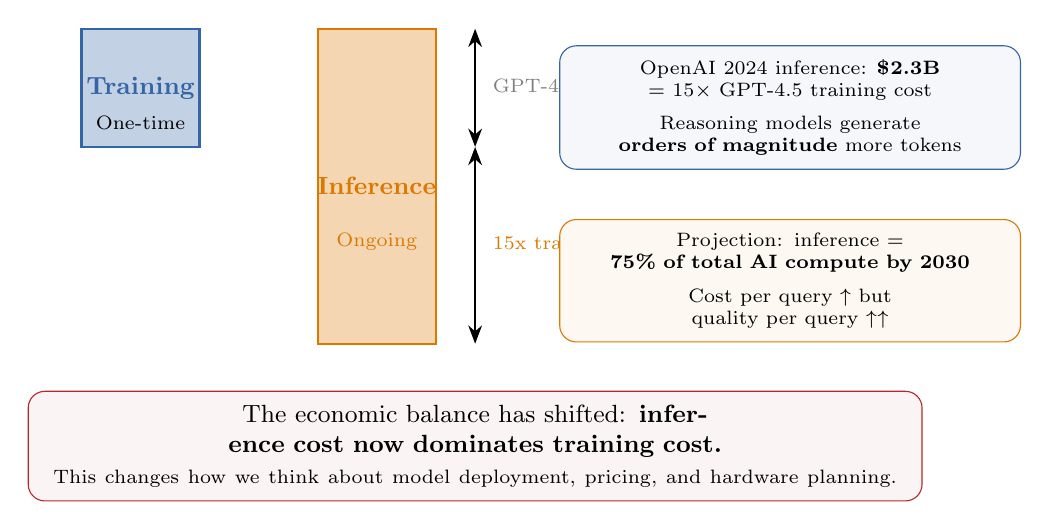
\begin{tikzpicture}
  % Training bar
  \fill[popblue!30] (-4, 2) rectangle (-2.5, 3.5);
  \draw[thick, popblue] (-4, 2) rectangle (-2.5, 3.5);
  \node[font=\small\bfseries, text=popblue] at (-3.25, 2.75) {Training};
  \node[font=\scriptsize] at (-3.25, 2.3) {One-time};

  % Inference bar (much taller)
  \fill[orange1!30] (-1, -0.5) rectangle (0.5, 3.5);
  \draw[thick, orange1] (-1, -0.5) rectangle (0.5, 3.5);
  \node[font=\small\bfseries, text=orange1] at (-0.25, 1.5) {Inference};
  \node[font=\scriptsize, text=orange1] at (-0.25, 0.8) {Ongoing};

  % Annotation
  \draw[thick, Stealth-Stealth] (1, 2) -- (1, 3.5);
  \node[font=\scriptsize, text=gray, right] at (1.1, 2.75) {GPT-4.5 training};
  \draw[thick, Stealth-Stealth] (1, -0.5) -- (1, 2);
  \node[font=\scriptsize, text=orange1, right] at (1.1, 0.75) {15x training cost};

  % Key numbers
  \node[draw=popblue, fill=popblue!5, rounded corners=6pt, text width=5.5cm, align=center, inner sep=5pt, font=\scriptsize] at (5, 2.5) {
    OpenAI 2024 inference: \textbf{\$2.3B}\\
    = 15$\times$ GPT-4.5 training cost\\[4pt]
    Reasoning models generate\\
    \textbf{orders of magnitude} more tokens
  };

  \node[draw=orange1, fill=orange1!5, rounded corners=6pt, text width=5.5cm, align=center, inner sep=5pt, font=\scriptsize] at (5, 0.3) {
    Projection: inference =\\
    \textbf{75\% of total AI compute by 2030}\\[4pt]
    Cost per query $\uparrow$ but\\
    quality per query $\uparrow\uparrow$
  };

  % Bottom
  \node[draw=warnred, fill=warnred!5, rounded corners=6pt, text width=11cm, align=center, inner sep=5pt, font=\small] at (1, -1.8) {
    The economic balance has shifted: \textbf{inference cost now dominates training cost.}\\
    {\scriptsize This changes how we think about model deployment, pricing, and hardware planning.}
  };
\end{tikzpicture}
\end{center}
\end{frame}

% ============================================================
% PRACTICAL GUIDE
% ============================================================
\begin{frame}
\frametitle{Practical guide}

\begin{center}
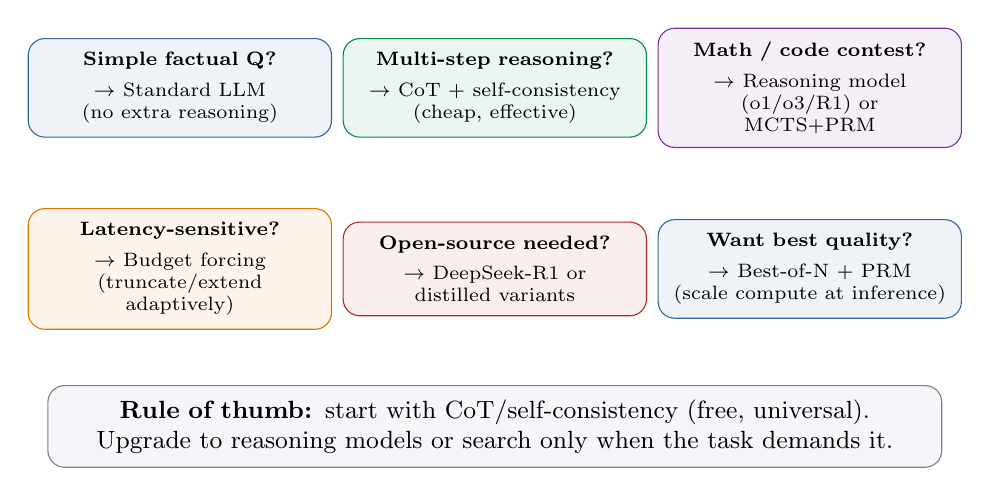
\begin{tikzpicture}
  % Decision nodes
  \node[draw=popblue, fill=popblue!8, rounded corners=6pt, text width=3.5cm, align=center, inner sep=5pt, font=\scriptsize] at (-4, 2.5) {
    \textbf{Simple factual Q?}\\[3pt]
    $\to$ Standard LLM\\(no extra reasoning)
  };

  \node[draw=paramgreen, fill=paramgreen!8, rounded corners=6pt, text width=3.5cm, align=center, inner sep=5pt, font=\scriptsize] at (0, 2.5) {
    \textbf{Multi-step reasoning?}\\[3pt]
    $\to$ CoT + self-consistency\\(cheap, effective)
  };

  \node[draw=violet1, fill=violet1!8, rounded corners=6pt, text width=3.5cm, align=center, inner sep=5pt, font=\scriptsize] at (4, 2.5) {
    \textbf{Math / code contest?}\\[3pt]
    $\to$ Reasoning model\\(o1/o3/R1) or MCTS+PRM
  };

  \node[draw=orange1, fill=orange1!8, rounded corners=6pt, text width=3.5cm, align=center, inner sep=5pt, font=\scriptsize] at (-4, 0.2) {
    \textbf{Latency-sensitive?}\\[3pt]
    $\to$ Budget forcing\\(truncate/extend adaptively)
  };

  \node[draw=warnred, fill=warnred!8, rounded corners=6pt, text width=3.5cm, align=center, inner sep=5pt, font=\scriptsize] at (0, 0.2) {
    \textbf{Open-source needed?}\\[3pt]
    $\to$ DeepSeek-R1 or\\distilled variants
  };

  \node[draw=popblue, fill=popblue!8, rounded corners=6pt, text width=3.5cm, align=center, inner sep=5pt, font=\scriptsize] at (4, 0.2) {
    \textbf{Want best quality?}\\[3pt]
    $\to$ Best-of-N + PRM\\(scale compute at inference)
  };

  % Bottom
  \node[draw=gray, fill=lightbg, rounded corners=6pt, text width=11cm, align=center, inner sep=5pt, font=\small] at (0, -1.8) {
    \textbf{Rule of thumb:} start with CoT/self-consistency (free, universal).\\
    Upgrade to reasoning models or search only when the task demands it.
  };
\end{tikzpicture}
\end{center}
\end{frame}

% ============================================================
% OPEN QUESTIONS
% ============================================================
\begin{frame}
\frametitle{Open questions}

\begin{center}
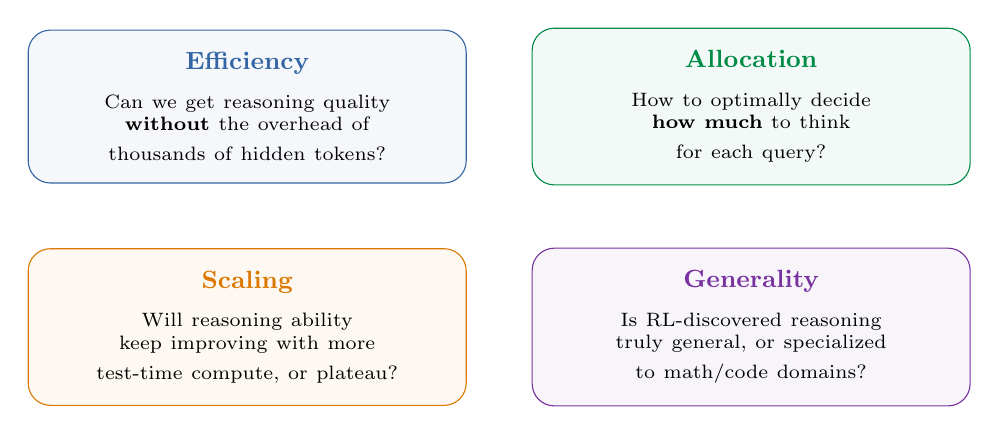
\begin{tikzpicture}
  \node[draw=popblue, fill=popblue!5, rounded corners=8pt, text width=5cm, align=center, inner sep=8pt, font=\small] at (-3.2, 2) {
    \textcolor{popblue}{\bfseries Efficiency}\\[6pt]
    {\scriptsize Can we get reasoning quality\\
    \textbf{without} the overhead of\\
    thousands of hidden tokens?}
  };

  \node[draw=paramgreen, fill=paramgreen!5, rounded corners=8pt, text width=5cm, align=center, inner sep=8pt, font=\small] at (3.2, 2) {
    \textcolor{paramgreen}{\bfseries Allocation}\\[6pt]
    {\scriptsize How to optimally decide\\
    \textbf{how much} to think\\
    for each query?}
  };

  \node[draw=orange1, fill=orange1!5, rounded corners=8pt, text width=5cm, align=center, inner sep=8pt, font=\small] at (-3.2, -0.8) {
    \textcolor{orange1}{\bfseries Scaling}\\[6pt]
    {\scriptsize Will reasoning ability\\
    keep improving with more\\
    test-time compute, or plateau?}
  };

  \node[draw=violet1, fill=violet1!5, rounded corners=8pt, text width=5cm, align=center, inner sep=8pt, font=\small] at (3.2, -0.8) {
    \textcolor{violet1}{\bfseries Generality}\\[6pt]
    {\scriptsize Is RL-discovered reasoning\\
    truly general, or specialized\\
    to math/code domains?}
  };
\end{tikzpicture}
\end{center}
\end{frame}

% ============================================================
% FURTHER READING
% ============================================================
\begin{frame}
\frametitle{Further reading}
\vspace{-0.3cm}
\begin{center}
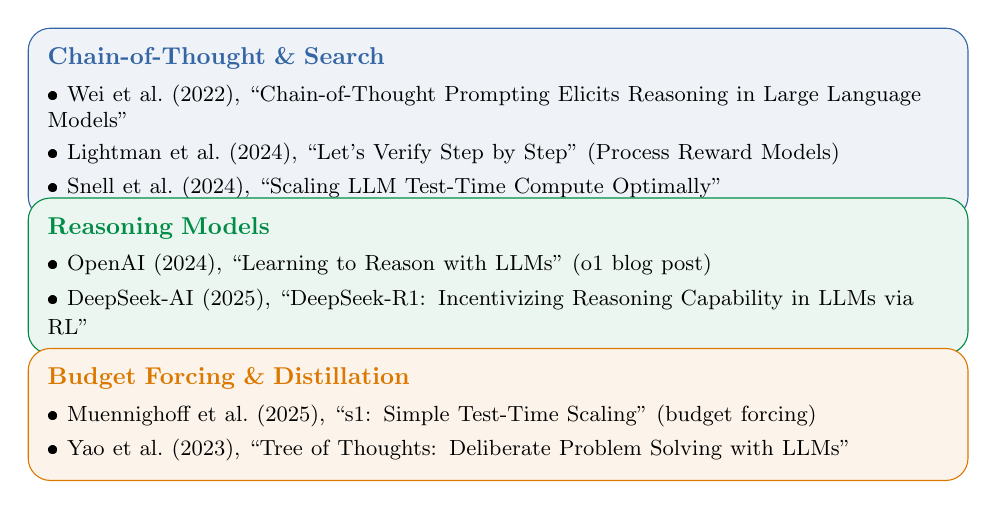
\begin{tikzpicture}[scale=0.88, transform shape]
  \node[draw=popblue, fill=popblue!8, rounded corners=8pt, text width=13cm, align=left, inner sep=8pt] at (0, 2.5) {
    \textbf{\textcolor{popblue}{Chain-of-Thought \& Search}}\\[4pt]
    {\small
    \textbullet~Wei et al.\ (2022), ``Chain-of-Thought Prompting Elicits Reasoning in Large Language Models''\\[2pt]
    \textbullet~Lightman et al.\ (2024), ``Let's Verify Step by Step'' (Process Reward Models)\\[2pt]
    \textbullet~Snell et al.\ (2024), ``Scaling LLM Test-Time Compute Optimally''
    }
  };
  \node[draw=paramgreen, fill=paramgreen!8, rounded corners=8pt, text width=13cm, align=left, inner sep=8pt] at (0, 0.3) {
    \textbf{\textcolor{paramgreen}{Reasoning Models}}\\[4pt]
    {\small
    \textbullet~OpenAI (2024), ``Learning to Reason with LLMs'' (o1 blog post)\\[2pt]
    \textbullet~DeepSeek-AI (2025), ``DeepSeek-R1: Incentivizing Reasoning Capability in LLMs via RL''
    }
  };
  \node[draw=orange1, fill=orange1!8, rounded corners=8pt, text width=13cm, align=left, inner sep=8pt] at (0, -1.7) {
    \textbf{\textcolor{orange1}{Budget Forcing \& Distillation}}\\[4pt]
    {\small
    \textbullet~Muennighoff et al.\ (2025), ``s1: Simple Test-Time Scaling'' (budget forcing)\\[2pt]
    \textbullet~Yao et al.\ (2023), ``Tree of Thoughts: Deliberate Problem Solving with LLMs''
    }
  };
\end{tikzpicture}
\end{center}
\end{frame}

% ============================================================
% QUESTIONS
% ============================================================
\begin{frame}
\begin{center}
\vspace{2cm}
{\Huge \textcolor{popblue}{Questions?}}

\vspace{1cm}
{\normalsize Next: Long Context \& Efficient Attention}
\end{center}
\end{frame}

\end{document}
